\documentclass [a4paper] {article}

\usepackage[spanish]{babel} 
\usepackage[utf8]{inputenc} 
\usepackage{multirow} 
\usepackage{float} 

\title{R-PL4}
\author{Gabriel López, Sergio Sanz, Álvaro Zamorano}

\usepackage{Sweave}
\begin{document}
\Sconcordance{concordance:G16-p4.tex:G16-p4.Rnw:%
1 10 1 1 0 32 1 1 2 1 0 1 1 14 0 1 2 7 1 1 2 1 0 1 1 8 0 1 2 3 1 1 2 10 %
0 1 2 3 1 1 2 24 0 1 2 8 1 1 2 15 0 1 2 2 1 1 2 1 0 1 1 3 0 1 2 3 1 1 2 %
10 0 1 1 10 0 1 2 7 1}


\maketitle

\graphicspath{ {./tmp/} }

\section{Ejercicio realizado en clase.}

\bigskip
A partir del siguiente conjunto de calificaciones académicas, pertenecientes a dos grupos de alumnos (mañana y tarde),
formados por dos notas: teoría y laboratorio, las notas de teoría y laboratorio tendrán valores entre 0 y 5, realizar
un análisis de clasificación no supervisada utilizando el algoritmo \textbf{K-Means}.

\begin{table}[H]
\begin{center}
\begin{tabular}{|c|c|c|c|c|}
\hline
Alumno & Teoría & Laboratorio\\
\hline \hline
A1 & 4 & 4 \\ \hline
A2 & 3 & 5 \\ \hline
A3 & 1 & 2 \\ \hline
A4 & 5 & 5 \\ \hline
A5 & 0 & 1 \\ \hline
A6 & 2 & 2 \\ \hline
A7 & 4 & 4 \\ \hline
A8 & 2 & 1 \\ \hline
\end{tabular}
\end{center}
\end{table}

En primer lugar se introducirán los datos en forma de matriz y se hará la traspuesta de esta.
\begin{Schunk}
\begin{Sinput}
> m<-matrix(c(4,4,3,5,1,2,5,5,0,1,2,2,4,5,2,1),2,8)
> (m<-t(m))
\end{Sinput}
\begin{Soutput}
     [,1] [,2]
[1,]    4    4
[2,]    3    5
[3,]    1    2
[4,]    5    5
[5,]    0    1
[6,]    2    2
[7,]    4    5
[8,]    2    1
\end{Soutput}
\end{Schunk}

\bigskip
En primer lugar se deben seleccionar el número de clusters en los que se van a agrupar los datos,
en este caso serán 2. Además es necesario indicar los centroides iniciales de cada uno de ellos, en
este caso son C1\{0,1\} y C2\{2,2\}. Todo ello es elegido de forma arbitraria.

\bigskip
Introducimos los centroides en una matriz y se realiza la traspuesta.
\begin{Schunk}
\begin{Sinput}
> c<-matrix(c(0,1,2,2),2,2)
> (c<-t(c))
\end{Sinput}
\begin{Soutput}
     [,1] [,2]
[1,]    0    1
[2,]    2    2
\end{Soutput}
\end{Schunk}

\bigskip
La función \texttt{K-Means} se encuentra en el paquete \textbf{stats}. Dicho paquete se carga por defecto al
arrancar R; para comprobarlo se hace uso de la función \texttt{search()}.
\begin{Schunk}
\begin{Sinput}
> search()
\end{Sinput}
\begin{Soutput}
 [1] ".GlobalEnv"        
 [2] "package:factoextra"
 [3] "package:ggplot2"   
 [4] "package:readr"     
 [5] "package:foreign"   
 [6] "package:stats"     
 [7] "package:graphics"  
 [8] "package:grDevices" 
 [9] "package:utils"     
[10] "package:datasets"  
[11] "package:methods"   
[12] "Autoloads"         
[13] "package:base"      
\end{Soutput}
\end{Schunk}

\bigskip
Por último hacemos uso de la función y obtenemos los centroides finales. Indicamos que el número máximo de
iteraciones es 4.
\begin{Schunk}
\begin{Sinput}
> (clasificacionns<-kmeans(m,c,4))
\end{Sinput}
\begin{Soutput}
K-means clustering with 2 clusters of sizes 4, 4

Cluster means:
  [,1] [,2]
1 1.25 1.50
2 4.00 4.75

Clustering vector:
[1] 2 2 1 2 1 1 2 1

Within cluster sum of squares by cluster:
[1] 3.75 2.75
 (between_SS / total_SS =  84.8 %)

Available components:

[1] "cluster"      "centers"     
[3] "totss"        "withinss"    
[5] "tot.withinss" "betweenss"   
[7] "size"         "iter"        
[9] "ifault"      
\end{Soutput}
\end{Schunk}

\bigskip
Los resultados obtenidos son los mismos que los de clase, es decir, \textbf{C1\{1.25,1.5\} y C2\{4,4.75\}.}

\bigskip
A continuación usaremos los clusters obtenios para separar los datos de la muestra en dos grupos. Para ello
se hace uso de la función \texttt{cbind} la cuál añade (por delante) una columna a la matriz de datos. Dicha
columna se corresponde con la clasificación obtenida, será 1 ó 2 dependiendo del cluster al que pertenezca
cada muestra.
\begin{Schunk}
\begin{Sinput}
> (m = cbind(clasificacionns$cluster,m)) 
\end{Sinput}
\begin{Soutput}
     [,1] [,2] [,3]
[1,]    2    4    4
[2,]    2    3    5
[3,]    1    1    2
[4,]    2    5    5
[5,]    1    0    1
[6,]    1    2    2
[7,]    2    4    5
[8,]    1    2    1
\end{Soutput}
\end{Schunk}

\bigskip
Una vez se tiene el cluster al que pertenece cada muestra, se separa la matriz siguiendo el criterio anterior.
\begin{Schunk}
\begin{Sinput}
> mc1=subset(m,m[,1]==1)
> mc2=subset(m,m[,1]==2)
\end{Sinput}
\end{Schunk}

\bigskip
Por último, limpiamos la columna introducida para el fin buscado y mostramos los dos conjuntos de datos
clusterizados.
\begin{Schunk}
\begin{Sinput}
> (mc1=mc1[,-1])
\end{Sinput}
\begin{Soutput}
     [,1] [,2]
[1,]    1    2
[2,]    0    1
[3,]    2    2
[4,]    2    1
\end{Soutput}
\begin{Sinput}
> (mc2=mc2[,-1])
\end{Sinput}
\begin{Soutput}
     [,1] [,2]
[1,]    4    4
[2,]    3    5
[3,]    5    5
[4,]    4    5
\end{Soutput}
\end{Schunk}

\bigskip
Se puede observar que las muestras 3,5,6,8 pertenecen al mismo grupo, mientras que las muestras 1,2,4,7 
se encuentran en el restante.

\section{Desarrollo por parte del alumno.}

\bigskip
En primer lugar hemos realizado un conjunto de funciones que realizan el algoritmo \textbf{K-Means}. Los parámetros
de esta función deben ser la matriz de muestras y la matriz con los centroides iniciales, al igual que se indica 
anteriormente. Como resultado, proporciona las coordenadas finales del centroide de cada uno de los clusters y varias
listas (número de clusters) incluyendo en cada una de ellas las muestras que pertenece a cada uno de los clusters.
Además, esta función, en caso de que los datos tengan 2 dimensiones, nos generará un gráfico donde se muestra la 
evolución del algoritmo a la largo de las diferentes iteraciones realizadas. 

Cabe destacar que el uso de la función se hace mediante matrices.

\bigskip
Procedemos a cargar dichas funciones.
\begin{Schunk}
\begin{Sinput}
> source("./Funciones/KMeans.R")
\end{Sinput}
\end{Schunk}

\bigskip
Las principales funciones codificadas son:
\begin{Schunk}
\begin{Sinput}
> calcularMatrizDistancias
\end{Sinput}
\begin{Soutput}
function (matrizMuestras, matrizCentroides,dimensiones) {
    sizeCentroides <- length(matrizCentroides)/dimensiones
    sizeMuestras <- length(matrizMuestras)/dimensiones
    x<-c()

    for (i in 1:sizeCentroides) {
        for (j in 1:sizeMuestras)
            x<-c(x,distanciaEuclidea(matrizCentroides[i,],matrizMuestras[j,]))
    }

    m<-matrix(x,nrow=sizeCentroides,ncol=sizeMuestras,byrow=T)

    return(m)
}
\end{Soutput}
\begin{Sinput}
> calcularMatrizPertenencia
\end{Sinput}
\begin{Soutput}
function (matrizDistancias, nCentroides) {
    sizeDistancias <- length(matrizDistancias)/nCentroides
    x<-c()

    for (i in 1:sizeDistancias) {
        posMinimo <- filaMinimo(matrizDistancias[,i])
        for (j in 1:nCentroides)
            if (j==posMinimo){
                x<-c(x,1)
            } else {
                x<-c(x,0)
            }
    }

    m<-matrix(x,nrow=nCentroides,ncol=sizeDistancias)

    return(m)
}
\end{Soutput}
\begin{Sinput}
> muestrasPorCluster
\end{Sinput}
\begin{Soutput}
function (matrizPertenencia, nCentroides) {
    sizeDistancias <- length(matrizPertenencia)/nCentroides
    finalList<-c()
    for (i in 1:nCentroides){
        finalList<-c(finalList, list(muestrasPorFila(matrizPertenencia[i,])))
    }
    
    m<-matrix(finalList,nrow=nCentroides,ncol=sizeDistancias)
    return(finalList)
}
\end{Soutput}
\begin{Sinput}
> obtenerMuestrasSeparadas
\end{Sinput}
\begin{Soutput}
function (matrizMuestras, muestrasPorCluster, dimensiones) {
    muestras<-t(matrizMuestras)
    sizeMuestras <- length(matrizMuestras)/dimensiones
    separadas<-list()

    for (i in 1:length(muestrasPorCluster)){
        nMuestrasCluster<-length(muestrasPorCluster[[i]])
        temp<-c()
        for (j in 1:sizeMuestras) {
            if (j %in% muestrasPorCluster[[i]]) {
                temp<-c(temp, muestras[,j])
            }
        }

        separadas[[i]]<-matrix(temp,nrow=dimensiones,ncol=nMuestrasCluster)
        
    }

    return(separadas)
}
\end{Soutput}
\begin{Sinput}
> obtenerNuevosCentroides
\end{Sinput}
\begin{Soutput}
function (muestrasSeparadas, dimensiones) {
    sizeMuestras <- length(muestrasSeparadas)
    centros<-c()

    for (i in 1:sizeMuestras){
        matriz<-muestrasSeparadas[[i]]
        centros<-c(centros,nuevoCentroide(t(matriz),dimensiones))
    }

    return(matrix(centros,nrow=sizeMuestras,ncol=dimensiones,byrow=T))
}
\end{Soutput}
\begin{Sinput}
> comprobarMatrizPertenencia
\end{Sinput}
\begin{Soutput}
function (matriz1, matriz2) {
    iguales<-TRUE
    i<-1

    while(iguales && i<=length(matriz1)){
        if (matriz1[i]==matriz2[i]){
            i<-i+1
        } else {
            iguales<-FALSE
        }
    }

    return(iguales)
}
\end{Soutput}
\end{Schunk}

\bigskip
Todas ellas se encuentran dentro de un bucle while realizado siempre y cuando cambie la matriz de pertenencia.

\bigskip
Respecto a la parte de \textbf{representación} se ha realizado otro conjunto de funciones con dicho fin. La
principal de ellas es:
\begin{Schunk}
\begin{Sinput}
> representar
\end{Sinput}
\begin{Soutput}
function(muestrasSeparadas,matrizMuestras,matrizCentroides,i){
    colores <- c("red","blue","green","black","purple")

    titulo<-paste("Iteracion ",i)

    m<-muestrasSeparadas[[1]]
    limites <- obtenerLimites(matrizMuestras)
    plot(m[1,],m[2,],pch=1,col=colores[1],xlim=limites$x,ylim=limites$y,
        main=titulo,xlab="X",ylab="Y")

    centroide<-matrizCentroides[1,]
    points(centroide[1],centroide[2],pch=8,col=colores[1])

    indiceColor <- 2

    nClusters<-length(muestrasSeparadas)
    for (i in 2:nClusters) {
        m<- muestrasSeparadas[[i]]
        points(m[1,],m[2,],pch=1,col=colores[i])

        centroide<-matrizCentroides[i,]
        points(centroide[1],centroide[2],pch=8,col=colores[indiceColor])

        indiceColor <- indiceColor + 1
        if (indiceColor==5) {
            indiceColor <- 1
        }
    }
}
\end{Soutput}
\end{Schunk}

\bigskip
Cabe indicar que únicamente se dispone de 5 colores diferentes, es decir, en caso de haber más de 5 clusters,
los colores de la gráfica volverían a repetirse.

\bigskip
Probamos nuestras funciones con los datos del apartado anterior y obtenemos la evolución del algoritmo.
\begin{Schunk}
\begin{Sinput}
> m<-t(matrix(c(4,4,3,5,1,2,5,5,0,1,2,2,4,5,2,1),2,8))
> c<-t(matrix(c(0,1,2,2),2,2))
> (resultado<-KMeans(m,c,"resultadoKMeans.png"))
\end{Sinput}
\begin{Soutput}
$centroides
     [,1] [,2]
[1,] 1.25 1.50
[2,] 4.00 4.75

$muestrasPorCluster
$muestrasPorCluster[[1]]
[1] 3 5 6 8

$muestrasPorCluster[[2]]
[1] 1 2 4 7
\end{Soutput}
\end{Schunk}
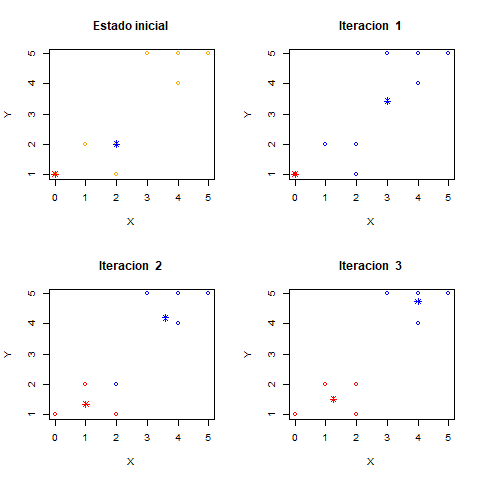
\includegraphics[width=\textwidth]{resultadoKMeans}

\bigskip
Se observa que los resultados obtenidos son los mismos que los conseguidos en clase.

\bigskip
Con el uso de estas funciones se realizará una clasterización no jerárquica de datos obtenidos de \texttt{Kaggle}
sobre información de diferentes países. Procedemos a leer dichos datos.

\bigskip
\begin{Schunk}
\begin{Sinput}
> library("readr")
> datos<-read.csv("./Datos/countries.csv")
\end{Sinput}
\end{Schunk}

\bigskip
Se usarán los datos porcentuales pertenecientes a los sectores de agricultura, industria y servicios para realizar
k-Means.

\bigskip
\begin{Schunk}
\begin{Sinput}
> datosEvaluar<-c(datos$Agriculture,datos$Industry,datos$Service)
> datosEvaluar<-matrix(datosEvaluar,15,3)
> cIniciales<-matrix(c(0.04,0.08,0.25,0.35,0.60,0.65),2,3)
> (resultado2<-KMeans(datosEvaluar,cIniciales,"resultadoKMeans.png"))
\end{Sinput}
\begin{Soutput}
$centroides
           [,1]      [,2]      [,3]
[1,] 0.02444444 0.2626667 0.7128889
[2,] 0.08916667 0.3988333 0.5121667

$muestrasPorCluster
$muestrasPorCluster[[1]]
[1]  2  3  4  5  7  8 10 14 15

$muestrasPorCluster[[2]]
[1]  1  6  9 11 12 13
\end{Soutput}
\end{Schunk}

\bigskip
A la vista de los resultados obtenidos, los países se clusterizan de la siguiente manera:
\begin{enumerate}
\item España, Portugal, Reino Unido, Estados Unidos, Alemania, Francia, Italia, Mexico, Canada
\item Argentina, Rusia, Brasil, China, Chile, Turquía
\end{enumerate}

Una de las diferencias de los países del primer cluster respecto a los restantes es el mayor 
porcentaje en el sector servicios y menor en el sector primario.

\bigskip
Con estos mismos datos realizaremos una clusterización \textbf{jerárquica} mediante el uso de los
paquetes \texttt{stats} y \texttt{factorextra}. Procedemos a cargar el segundo de ellos.
\begin{Schunk}
\begin{Sinput}
> install.packages("factoextra")
> library(factoextra)
\end{Sinput}
\end{Schunk}

\bigskip
Previo a la clusterización es necesario escalar los datos mediante la función \texttt{scale.}
\begin{Schunk}
\begin{Sinput}
> datosCJ<-scale(datosEvaluar)
\end{Sinput}
\end{Schunk}

\bigskip
Por último, usando la función \texttt{hclust} se realiza dicha clusterización.
\begin{Schunk}
\begin{Sinput}
> hCJ<-hclust(d = dist(x=datosCJ, method="euclidean"), method="complete")
\end{Sinput}
\end{Schunk}

\bigskip
Para mostrar los resultados obtenidos se usa una función definida por nosotros y así poder pasar estos
a un formato de foto. Es necesario indicar el número de clusters que queremos obtener.
\begin{Schunk}
\begin{Sinput}
> source("./Funciones/representarCJ.R")
> representarCJ(hCJ,2,"resultadoCJ.png")
\end{Sinput}
\end{Schunk}

\includegraphics[width=\textwidth]{resultadoCJ}

\bigskip
Se puede observar que la clusterización de países se corresponde con la obtenida anteriormente mediante
el uso de KMeans.

\end{document}
